\documentclass[11pt]{article}\usepackage{knitr}

%AMS-TeX packages
\usepackage{amssymb,amsmath,amsthm} 
%geometry (sets margin) and other useful packages
\usepackage[margin=1in]{geometry}
\usepackage{graphicx, ctable, booktabs}
\usepackage{color}
\usepackage{listings}
\usepackage{ltablex, calc, enumerate, multirow, float, soul, paralist}
\usepackage{hyperref}
\usepackage{longtable, pdflscape, textcase}
\usepackage[backend=bibtex, natbib=true]{biblatex}
\addbibresource{references/refs.bib}
\IfFileExists{upquote.sty}{\usepackage{upquote}}{}

\begin{document}









\setlength{\parskip}{3ex}
\setlength{\parindent}{0pt}

\title{Putting Down Roots: A Graphical Exploration of Community Attachment}
\author{Andee Kaplan, Eric Hare}

\maketitle

\setcounter{page}{1}
\section*{Introduction}

This is the introduction.

\subsection*{Philosophy}
The goal of our work is to facilitate understanding of why people feel attachment to their communities through the use of an interactive and web-based approach. Specifically, we took the point of view of a community planner, either from one of the communities in the study or from a community in the same region or a similar urbanicity. By putting the user in the driver seat of their own experience, we allow the user to apply the conclusions of their interaction to their own situation.


\section*{Technology}

In order to explore the dataset we first created an interactive tool to facilitate the emergence of interesting or descriptive patterns. The construction and design of this tool are detailed in the following sections.

\subsection*{Description and Design}
The interactive tool is comprised of three pieces, \begin{inparaenum}[\itshape 1\upshape)]
\item Control panel, 
\item Map Panel, and
\item Plot panel.
\end{inparaenum}
As the user interacts with each piece, the remaining portions of the interface update to reflect the interaction. In this way we have built an interactive graphic, rather than an animation.

\begin{figure}[H]
\centering
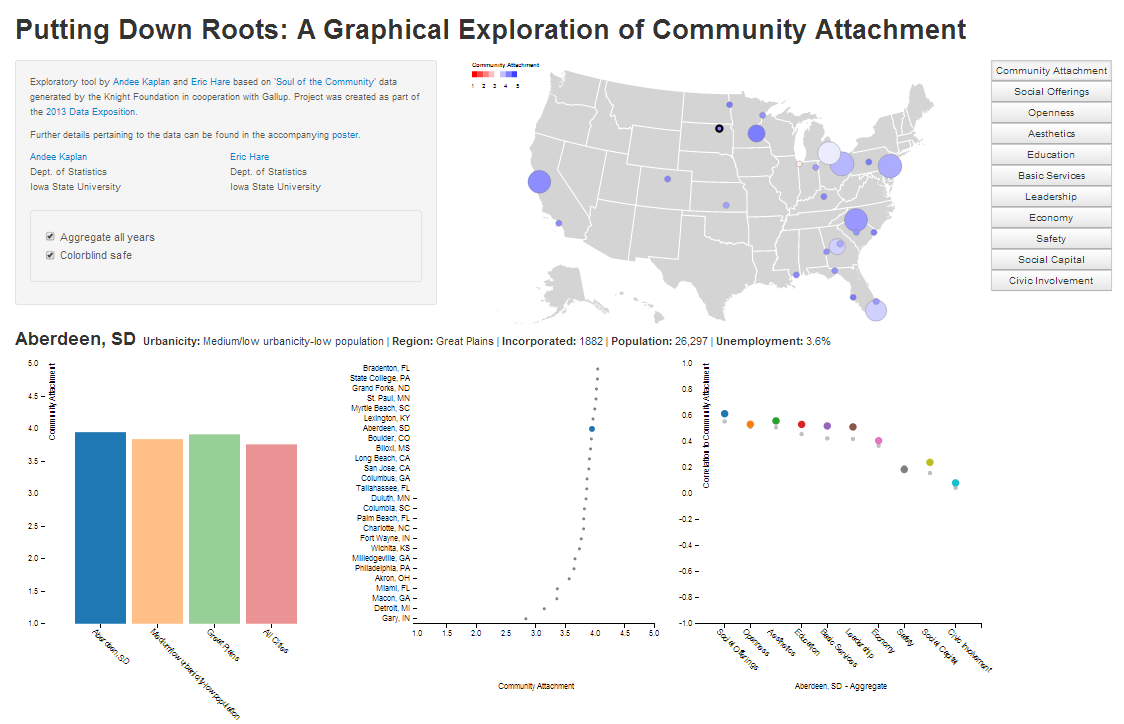
\includegraphics[width=\textwidth]{images/tool.png}
\caption{\label{fig:tool} The components that make up the interactive web interface, (1) Control panel, (2) Map panel, and (3) Plot panel.}
\end{figure}



\subsection*{The Shoulders of Giants}

\subsection*{Why?}
During the creation of our interactive tool, we found it useful to stop and ask, ``Why?'' This process enabled the type of introspection necessary to help ensure usability and relevance in a project of this type.

\subsubsection*{Interactive}
Why interactive? In order to discover what the data has to tell the world. In the words of John Tukey, "Exploratory data analysis is detective work - numerical detective work - or counting detective work - or \emph{graphical detective work}." \cite{tukey77} Dynamic, interactive visualizations can empower people to explore the data for themselves as well as encourage engagement with the data in a way that static visualizations cannot.

\subsubsection*{Linked Plots}
Why linked plots? Linking multiple visualizations shows different aspects of a complex data set and helps highlight relationships. By allowing actions in one plot to affect elements in other plots, comparisons are made easy for the user without requiring much memorization. This aids in pattern finding by avoiding taxation of the user's brain through memorization.

\subsubsection*{Web-based}
Why web-based? A web-based application is platform-independent and allows the user to employ the tool without any software to download. Additionally, by building an application that works on all modern browsers and operating systems, there are no limitations on who can use the tool. Finally, automatic feature additions and bug fixes can be completed transparently to the user.


\section*{Stories}

We elected to divide our analysis using two primary factors. The first is the geographic region the community is located in, and the second is the urbanicity of the particular community. Urbanicity is a census designation which was provided in the dataset, while regions were determined by us. The regions are a rough guideline and do not correspond to any commonly used or accepted regional boundaries. They were merely a method we used to cluster communities into more-alike regions in terms of geography and culture. The interactive tool was then used to help us discover a story in the data for each of the five regions.

\subsection*{Great Plains}
\begin{knitrout}
\definecolor{shadecolor}{rgb}{0.969, 0.969, 0.969}\color{fgcolor}\begin{figure}[H]

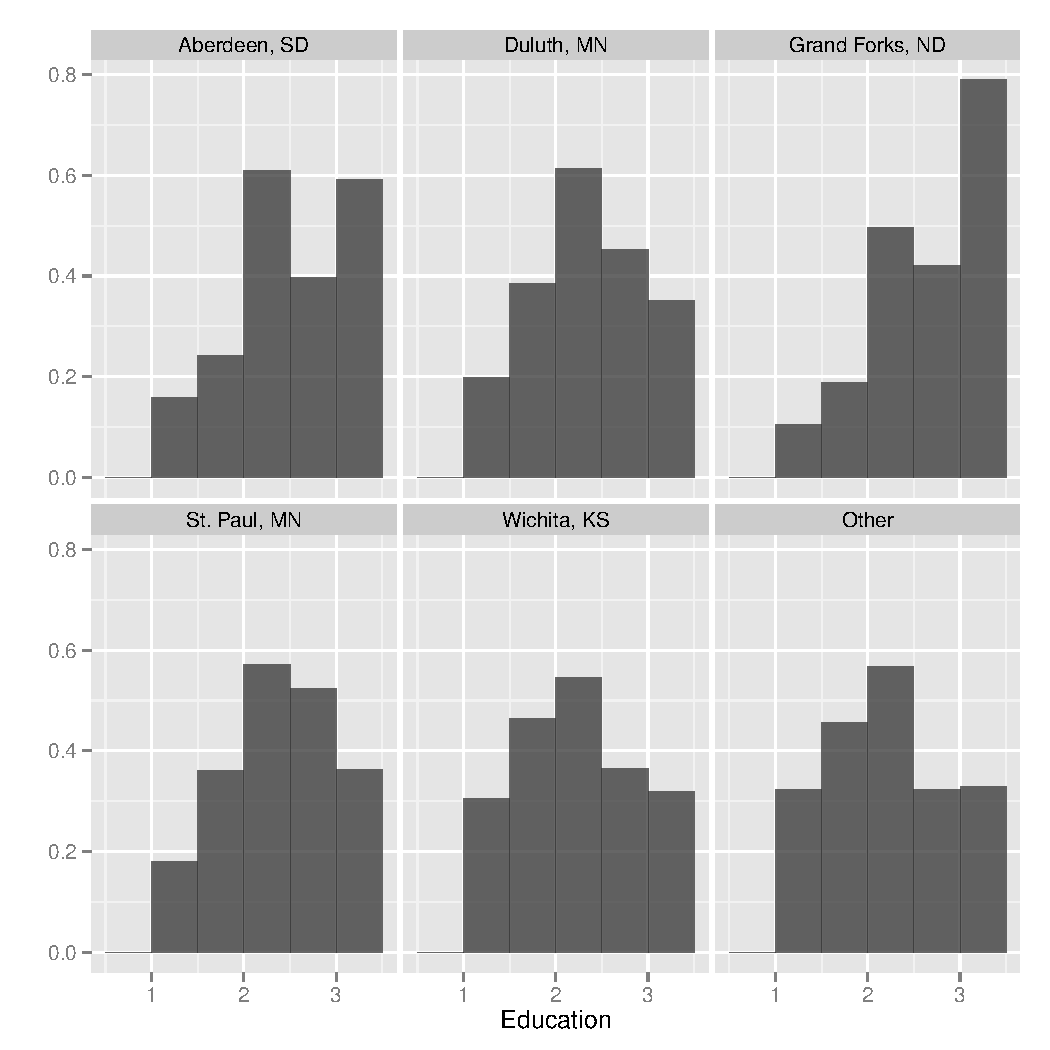
\includegraphics[width=\maxwidth]{figure/gp_one} \caption[Caption]{Caption...\label{fig:gp_one}}
\end{figure}


\end{knitrout}


\begin{knitrout}
\definecolor{shadecolor}{rgb}{0.969, 0.969, 0.969}\color{fgcolor}\begin{figure}[H]

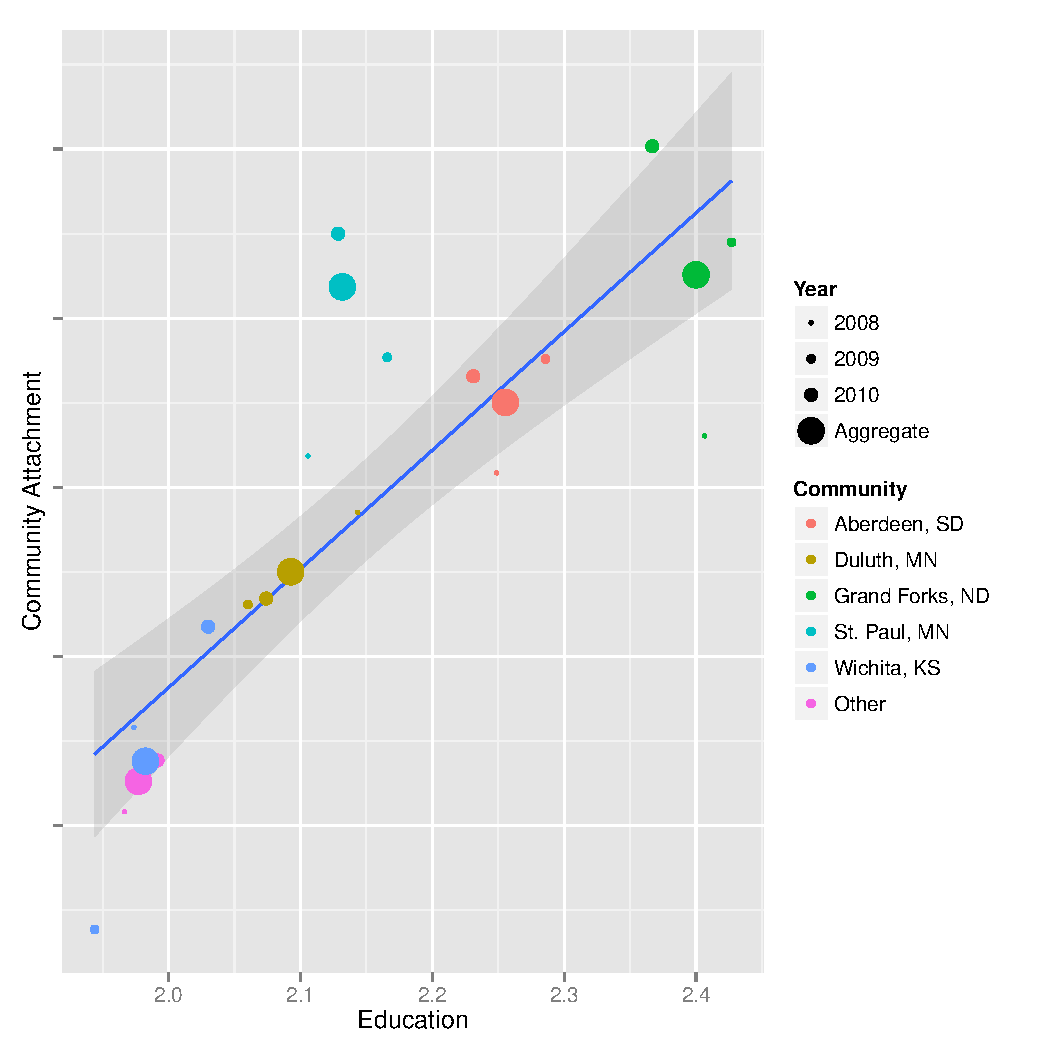
\includegraphics[width=\maxwidth]{figure/gp_two} \caption[Caption]{Caption...\label{fig:gp_two}}
\end{figure}


\end{knitrout}



\subsection*{West}
\begin{knitrout}
\definecolor{shadecolor}{rgb}{0.969, 0.969, 0.969}\color{fgcolor}\begin{figure}[H]

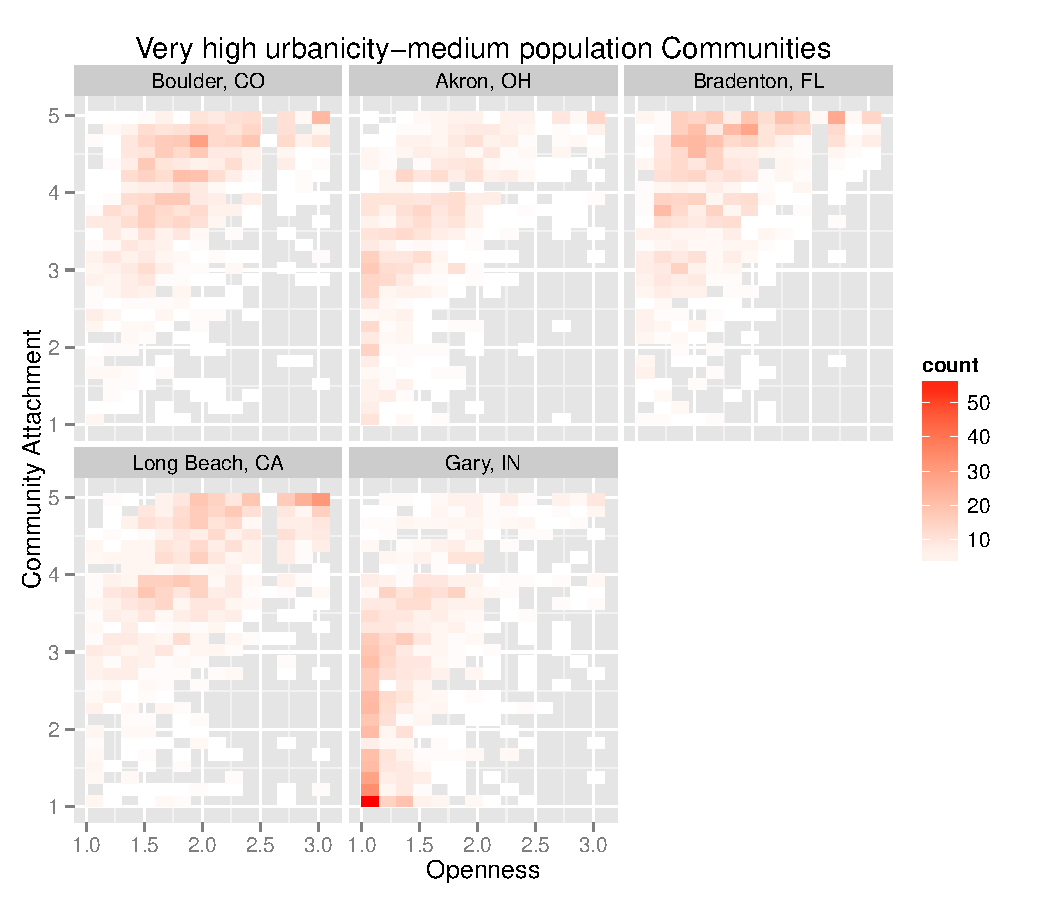
\includegraphics[width=\maxwidth]{figure/west_one} \caption[Caption]{Caption...\label{fig:west_one}}
\end{figure}


\end{knitrout}



\subsection*{Deep South}
\begin{knitrout}
\definecolor{shadecolor}{rgb}{0.969, 0.969, 0.969}\color{fgcolor}\begin{figure}[H]

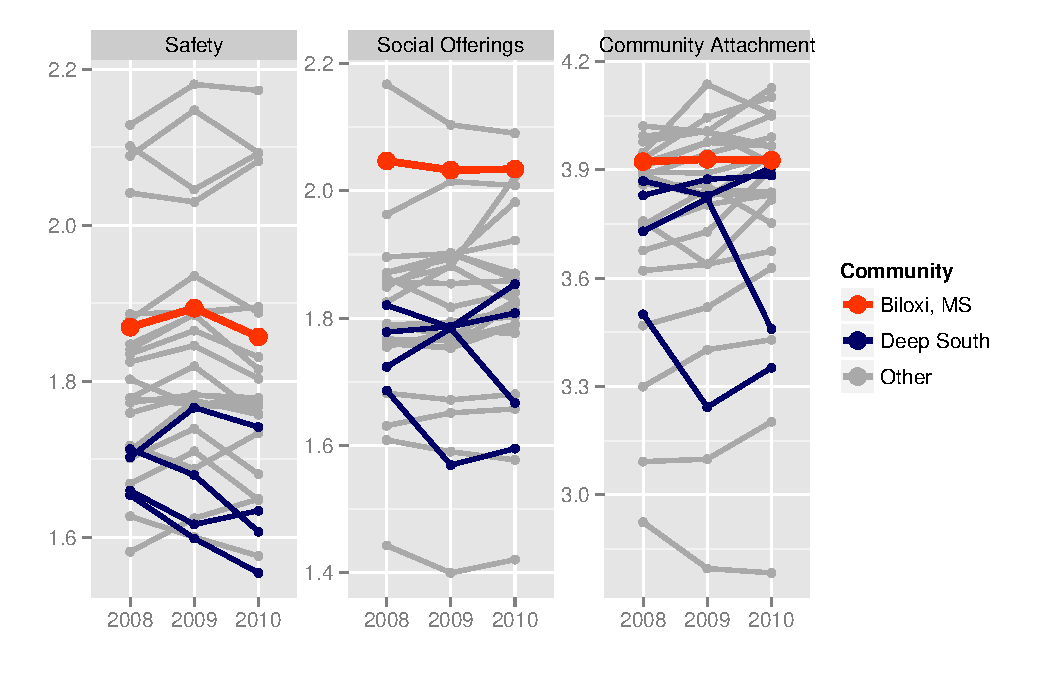
\includegraphics[width=\maxwidth]{figure/ds_one} \caption[Caption]{Caption...\label{fig:ds_one}}
\end{figure}


\end{knitrout}


\subsection*{Southeast}
\begin{knitrout}
\definecolor{shadecolor}{rgb}{0.969, 0.969, 0.969}\color{fgcolor}\begin{figure}[H]

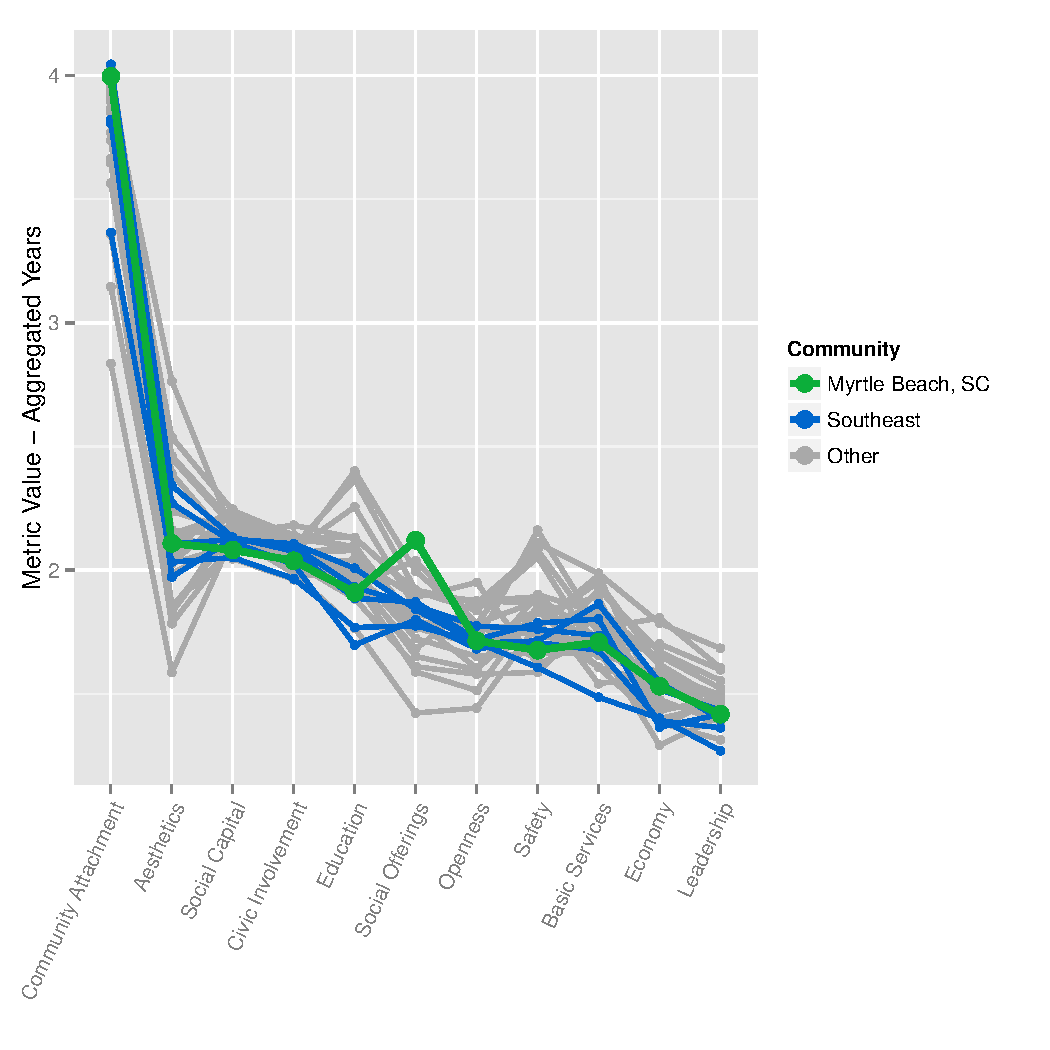
\includegraphics[width=\maxwidth]{figure/southeast_one} \caption[Mean value of metric for each community]{Mean value of metric for each community. Myrtle Beach is highlighted in green, and the other communities in the Southeast are highlighted in blue.\label{fig:southeast_one}}
\end{figure}


\end{knitrout}


\subsection*{Rust Belt}
\begin{knitrout}
\definecolor{shadecolor}{rgb}{0.969, 0.969, 0.969}\color{fgcolor}\begin{figure}[H]

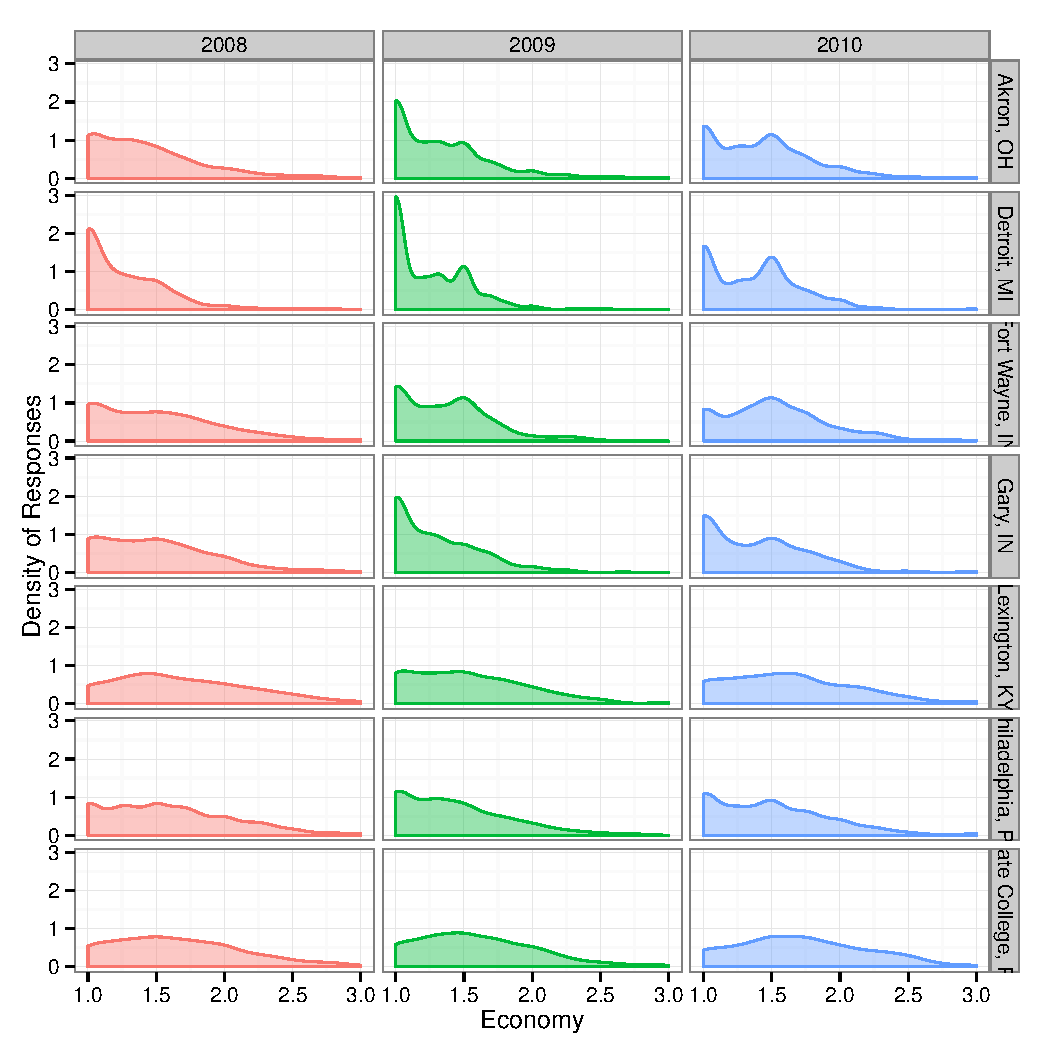
\includegraphics[width=\maxwidth]{figure/rb_one} \caption[Caption]{Caption...\label{fig:rb_one}}
\end{figure}


\end{knitrout}



\section*{Conclusion}

This is the conclusion.


\printbibliography
\end{document}
